\documentclass{article}
\usepackage[utf8]{inputenc}
\usepackage[T1]{fontenc}
\usepackage{microtype}
\usepackage{graphicx}
\usepackage{booktabs}
\usepackage{amsmath,amssymb,amsthm}
\usepackage{array}
\usepackage{placeins}
\usepackage{url}
\usepackage[hyperfootnotes=false]{hyperref}
\usepackage[preprint]{icml2026}
\hypersetup{pdftitle={Evidence Before Inference: Intent-Conditioned Language Support with Replayable Observations},pdfauthor={Anonymous Authors},pdfsubject={Research prototype and synthetic evaluation; not submitted or peer reviewed},colorlinks=true,urlcolor=blue,citecolor=blue,linkcolor=blue}
\icmltitlerunning{Evidence Before Inference}
\icmlkeywords{learner modeling, observation provenance, language learning, synthetic evaluation, diagnostic policy}
\newtheorem{proposition}{Proposition}
\newcommand{\Nabu}{\textsc{Nabu}}
\newcommand{\ind}{\mathbf{1}}
\newcommand{\artifact}[1]{\nolinkurl{#1}}
% The official style files are unmodified. This anonymous preprint has no
% invented affiliation, address, author identity, or conference-submission claim.
\makeatletter
\renewcommand{\printAffiliationsAndNotice}[1]{%
  \global\icml@noticeprintedtrue%
  {\let\thefootnote\relax\footnotetext{\hspace*{-\footnotesep}%
  Anonymous research prototype. Not submitted or peer reviewed.
  All reported learner outcomes are synthetic.}}}
\makeatother

\begin{document}
\twocolumn[
\icmltitle{\texorpdfstring{Evidence Before Inference:\\Intent-Conditioned Language Support with Replayable Observations}{Evidence Before Inference: Intent-Conditioned Language Support with Replayable Observations}}
\begin{icmlauthorlist}
\textbf{Anonymous Authors}
\end{icmlauthorlist}
\vskip 0.3in
]
\printAffiliationsAndNotice{}

\begin{abstract}
A language assistant can know what a learner is trying to do without knowing what that learner can do unaided. We extend the existing \Nabu{} reader with scoped intents, a conservative structural adapter, and an optional evidence loop that preserves the source activity. The loop records immutable, versioned observations and exposes replayable, condition-specific assessments; it does not convert exposure, assistance, or structural relationships into mastery. We formalize scoped replay invariance and a simple nonidentifiability boundary, then evaluate representation, prediction, and policy separately using a reproducible synthetic protocol. Structural borrowing improves new-family Brier score from .2500 to .1162 when a shared operation is assumed, but worsens it to .5195 under a wrong applicability domain; an outcome-sensitive policy also changes from helpful to harmful as the shared time budget increases. These counterexamples support an auditable separation of evidence and inference, not a claim of human learning benefit or a validated learner model.
\end{abstract}

\section{Introduction}
\label{sec:introduction}

A person reading a message may want to understand one command, prepare for a conversation, or simply explore. These intentions determine what help is relevant. They do not establish whether the person recognizes a word, can retrieve its form, can apply a grammatical operation to another base, or will succeed in a different context tomorrow. A useful language assistant must keep these distinctions even when its interface makes help immediate.

Consider an observed success after the learner has opened a translation. It is a real interaction and may be useful to the learner. Counting it as unaided production would make a stronger claim than the observation supports. A repeated display supplies opportunities to notice a form, but not observed recognition. A skip can occur because the learner already knows an answer, does not know it, or wants to keep reading. Likewise, a relation between forms can be linguistically appropriate while a learner has memorized those forms independently.

This paper asks: \emph{what should an intent-aware language assistant record and expose before it claims to infer competence or chooses a diagnostic interruption?} We address the question as a constrained extension of \Nabu{}, an existing language reader and exercise application. We retain its content, public identifiers, storage mechanisms, and scheduler. The implementation separates an immediate learner activity from an optional destination and from an organization's objective; separates authored language structure from observed responses; and offers short checks only where their outcomes can change the next help.

The contribution is an executable evidence contract and an evaluation design that makes failure visible. First, a versioned observation envelope preserves actor, source occurrence, task, assistance, response, and scoring provenance. A deterministic replay produces bounded direct counts and an inspectable ledger, while overall competence remains unknown. Second, a small authored contrast sequence exercises the contract inside the reader without changing existing spaced-repetition schedules. Third, matched synthetic comparisons isolate structural assumptions in prediction from action selection under a fixed budget. The experiments include independent memorization, misleading applicability, stale histories, and policy reversals rather than only a world in which transfer is correct.

We make no claim of a new knowledge-tracing algorithm, a complete language ontology, or measured instructional effectiveness. The prototype and generated experiments establish narrower properties: which evidence receives assessment credit, which assumptions produce predictive gains or failures, and why fewer questions need not imply better outcomes. The code and all generated results accompany the paper.

\section{Setting and Related Work}
\label{sec:setting}

\paragraph{Existing system.}
The inspected repository uses browser-native JavaScript modules, a FastAPI/Pydantic server, SQLite, and an existing IndexedDB content store for guests. Its scheduler is SM-2-inspired with separate practice modes. The bank contains 1,026 authored alignment entries across 12 languages; curated content supplies six Arabic pieces, 24 annotations, and 18 legacy activities. These are repository facts, not corpus statistics or independent linguistic validation. Alignment identifiers are preserved as alignment identifiers, not relabeled as true multilingual lexemes. The additions do not replace the reader, bank, or scheduler.

\paragraph{Intent and ownership.}
An intent records an immediate activity, optional destination and horizon, language and modality, optional source references, preferences, lifecycle, and field provenance. Explicit, inferred, exploratory, and unknown information remain distinguishable. A conservative local parser preserves the original text and leaves unsupported details unknown. An individual or team may have an open-ended activity with no destination. A team objective is stored separately from each member's private immediate intent. Actor and tenant checks operate through the existing authenticated backend; guest data use the existing local store. This is application-level scoping in the current infrastructure, not a claim of audited enterprise isolation.

\paragraph{Learner modeling.}
Knowledge tracing models latent acquisition through a probabilistic observation and learning process \citep{corbett1994knowledge}. Performance Factors Analysis uses success and failure histories for performance prediction and adaptive practice \citep{pavlik2009performance}. Half-life regression models recall over time using fitted spaced-repetition parameters \citep{settles2016trainable}. These approaches motivate being explicit about the link between behavior and a latent state. Our production projection does not fit or instantiate these models. It returns a provenance-preserving account of direct evidence; the separate Beta models below are deliberately small, assumed research models.

\paragraph{Evaluation.}
We distinguish a proper probability score from bin-based calibration summaries. The binary Brier score measures squared probabilistic error \citep{brier1950verification}; proper scoring rules provide a principled basis for comparing forecasts \citep{gneiting2007proper}. Calibration is a different property, and binning choices matter \citep{guo2017calibration}. Our simulation illustrates this distinction: an uninformative constant prediction can have lower aggregate calibration error than a more discriminating but underconfident predictor. None of these citations constitutes empirical validation of the new \Nabu{} features.

\section{An Evidence Contract Before a Learner Model}
\label{sec:contract}

\subsection{Three Separate Objects}

The implementation keeps three kinds of claims apart (Table~\ref{tab:layers}). A structural record may describe a form, provisional reading, authored usage, media anchor, or complete pattern application. It is not an observation of a person. An observation records what occurred under particular conditions. A policy chooses among available help, a check, and continuation; its usefulness remains a hypothesis until evaluated.

\begin{table}[t]
\caption{The implemented separation. A record in one layer does not silently become evidence in another.}
\label{tab:layers}
\centering
\begin{tabular}{@{}>{\raggedright\arraybackslash}p{.22\columnwidth}>{\raggedright\arraybackslash}p{.33\columnwidth}>{\raggedright\arraybackslash}p{.34\columnwidth}@{}}
\toprule
Layer & Retained evidence & Unsupported leap \\
\midrule
Structure & Language, reading, application, provenance, review status & A related form is known by this learner \\
Observation & Exact task, response, cues, attempt, source, scorer & Exposure or assisted success is mastery \\
Policy & Available action, intended use, conditional branches, interruption & A chosen action has measured learning gain \\
\bottomrule
\end{tabular}
\end{table}

The structural adapter preserves legacy identifiers and marks provisional per-language readings explicitly. Generated or quarantined material does not become an attested candidate. A full pattern application must retain its inputs, outputs, features, provenance, and competing analyses together. Multiple outputs from one application remain one provenance lineage. No production morphology dataset is imported in this release, and no missing annotation-to-concept links are invented.

\subsection{Versioned Observations and Conditions}

An event is an immutable record $e=(\mathrm{id},t,a,\eta)$, where $a$ is the user/team scope and $\eta$ contains the versioned envelope. The envelope binds an episode and attempt to the exact content version and occurrence, reading and context references, task version, input/output modalities, response or skip, assistance flags, and rubric/scorer/analysis references. Intent and organization-objective revisions are references, not copies of sensitive free text.

The four evidence dimensions are visual recognition, auditory recognition, retrieval, and contextual production. They are distinct from the existing recognition, listening, production, and cloze practice modes. The ledger retains both. A multiple-choice recognition response never silently becomes free production. A text-only task does not establish listening. The schema supports audio observations, but this release has no newly authored audio assessment because no appropriate curated recording was available.

Assistance is explicit: lookup, hint, answer, translation, replay, feedback, supplied base meaning, visible source, and other support. Replay reconciles recorded help within the episode and retry lineage; mandatory assistance specified by a task also overrides an incomplete client declaration. The ledger retains assistance sources and the exact conditions. A new sentence identifier alone does not establish a changed linguistic condition. Delayed-condition records report the actual elapsed time and explicitly changed lexical, sense, speaker, or syntactic fields, with unknown fields retained as unknown.

\subsection{A Conservative Projection}

Let $\Pi_{a,t,R}(E)$ be the projection of events $E$ for actor $a$ at replay time $t$, using a fixed, pure task resolver and scorer $R$. Its ledger retains observations even when they cannot be assessed. An aggregation key is
\begin{equation}
 k=(\text{target},\text{evidence dimension},\text{practice mode}).
\end{equation}
Context remains in individual ledger rows; aggregation at $k$ does not imply that contexts or episodes are statistically independent.

For a response $e$, define $A(e)=1$ only if the exact task resolves, the current admissible scorer returns a binary assessment, $e$ is the uniquely earliest response for its root episode and $k$, the response is unaided, it is not a retry or unresolved lineage, and $e.t\leq t$. Tied earliest timestamps abstain instead of using event-ID order as evidence of which answer came first. Then direct assessment counts are
\begin{align}
 c_k^+ &= \sum_{e:k(e)=k} A(e)\ind[y(e)=1],\\
 c_k^- &= \sum_{e:k(e)=k} A(e)\ind[y(e)=0].
\end{align}
Unknown, unscored, quarantined, or changed scoring references contribute to neither count. An explicitly requested rescore can reinterpret a preserved event with new references; default replay refuses this silent substitution. A seven-day freshness window and a 24-hour delayed-check threshold are fixed review policies, not fitted forgetting parameters. Counts are an audit summary; the returned \artifact{competence} field remains \artifact{null}.

\begin{proposition}[Scoped replay invariance]
\label{prop:replay}
Fix the selected actor, replay time, thresholds, resolver/scorer, and rescore option. For validated enveloped events accepted by the scoped sequence validator, permutation and insertion of exact canonical duplicates do not change $\Pi$. Conflicting payloads with the same in-scope identifier are rejected.
\end{proposition}
\begin{proof}
Scope selection and canonical payload equality determine a unique record per identifier. Sequence validation fixes episode and retry relationships. Sorting, assistance reconciliation, earliest-response tie detection, reference resolution, and aggregation are deterministic functions of that unique set. Therefore neither input order nor multiplicity of identical records changes the projection. Conflicts fail before projection. The claim excludes unenveloped legacy records, whose ignored-record audit counter may change under duplication.
\end{proof}

This is not a monotonicity claim. Adding a previously missing help event can correctly remove unaided assessment credit. It is also not tamper-proof behavioral measurement: server scoping and validation cannot establish that a person actually refrained from external help.

\begin{proposition}[Passive evidence does not identify competence]
\label{prop:nonidentifiable}
Without an additional behavioral model or assessed response, a fixed structural graph, intent, and passive observation sequence need not identify the probability of an unaided future response.
\end{proposition}
\begin{proof}
Construct two worlds with identical graph, intent, and 50 displayed occurrences, generated independently of response ability. In one world a future unaided response is Bernoulli$(.1)$; in the other it is Bernoulli$(.9)$. The observed inputs are identical, so any estimator using only these inputs returns the same value in both worlds and cannot identify both probabilities. The same construction applies to an unmodeled skip. A justified behavioral model could add assumptions; the event alone does not supply them.
\end{proof}

\section{Optional, Decision-Sensitive Checks}
\label{sec:policy}

The reader exposes immediate help, an optional check, and continuation. The chosen media and existing card/log nodes are preserved. An opted-in check covers the source and background content and stops device pronunciation to avoid treating a visible answer as unaided recall. Reopening in the same actor, intent revision, and content scope within a fixed 30-minute operational window resumes the episode and its assistance history. A new window does not establish statistical independence. A request to avoid practice suppresses checks. The existing task-aware recommendation remains the entry point; no graph posterior or reward-learning agent is introduced.

Eight authored contrast tasks surround an existing Arabic command phrase. They separate base-meaning recognition, a supplied-meaning form contrast, another-base recognition, application on that base, the opposite address direction, a further supplied-meaning base, an immediate phrase completion, and a delayed sentence check. The other-base application requires direct evidence about that base's meaning; a supplied meaning is recorded as assistance. These drafts are not instructor-validated linguistic assessments. They make competing explanations visible: a mismatch can reflect lexical difficulty, an operation difficulty, a misread instruction, or a slip. It does not identify one cause.

The production policy uses transparent branches. If base meaning already mismatches, it offers that meaning immediately rather than asking more questions merely to reduce uncertainty. Where outcomes change the next help, a check can be offered. The authored 30-second check budget is a design label, not a measured response time. Intent determines relevance and interruption preferences; it is not a prior score of competence.

The following elementary decision property explains the branch requirement, without asserting that the heuristic is optimal. Let $H$ be current history, $Y$ a question's possible response, and $U(a)$ the utility of a subsequent action. If one action $a^*$ maximizes $\mathbb E[U(a)\mid H,Y=y]$ for every possible $y$, and the question has no learning or intrinsic utility, then
\begin{equation}
\mathbb E_Y\!\left[\max_a\mathbb E[U(a)\mid H,Y]\right]
=\mathbb E[U(a^*)\mid H].
\end{equation}
The equality follows by substituting $a^*$ and iterated expectation. The decision value of that question is zero; a positive interruption cost makes it worse. Outcome-dependent actions are therefore necessary under these assumptions, but not sufficient for useful questioning. Direct help can be valuable for a known, low-uncertainty gap.

\section{Evaluation Protocol}
\label{sec:evaluation}

All reported experiments are generated by \artifact{tools/evaluate_evidence.mjs}, protocol \artifact{synthetic-evidence-v1}. They use 12 declared seeds and 128 fictional learners per seed and world. No parameters are fitted, no seeds are selected for favorable outcomes, and no natural-language benchmark or human observation is used. Means and sample standard deviations describe variation across these fixed-seed replicate means, not confidence intervals about people.

We separate three questions. \emph{Representation} checks complete records, distinct readings, provenance grouping, and split integrity. \emph{Prediction} compares two models on identical observations and held-out questions. \emph{Policy} compares two action rules with the same estimator, content pool, time costs, and budget. Changing all three at once would prevent attribution.

\subsection{Representation and Semantic Checks}

A fictional complete application is passed through the production structural validator. Its three outputs share one source lineage. Twelve lexical-family identifiers are assigned independently of surface spelling or suffixes. Six families are observed, and six are held out wholesale; the family intersection is zero. Shape validation does not certify linguistic correctness.

Nine synthetic observation cases test repeated displays, lookups, pronunciation playback, both knowing and unknowing skips, an assisted retry after failure, exact duplication, assisted-only success, and a later independent response. The research selector and the real production projector are checked separately. All nine production semantic checks pass with competence unknown. Fifty passive events produce zero assessed successes or failures. An unaided failure followed by an assisted correct retry remains one failure and zero successes; a later independent assessed success can add one success.

\subsection{Matched Prediction Comparison}

Each family has three distinct output identities, $a,b,c$. Training supplies three independently generated assessed episodes for $a,b$ in each of the six observed families: 36 responses per fictional learner. Evaluation contains 12 later responses to trained items, six new $c$ items within observed families, and six $a$ items from entirely held-out families. There are 36,864 distinct held-out outcomes per world, shared by both estimators. Held-out outcomes never update a model before scoring.

The direct estimator is research-only Beta$(1,1)$ at the exact item and practice mode. With $s$ successes and $n$ accepted assessments,
\begin{equation}
 p_D=(1+s)/(2+n).
\end{equation}
The experimental graph-informed estimator keeps these direct counts unchanged. It selects at most one observed result from each other declared family sharing the stipulated operation, reading, and mode. The target family is excluded. With at least three eligible families, it forms
\begin{align}
 p_F&=(1+s_F)/(2+n_F),\\
 w&=\min\{.85,4/(4+n)\},\\
 p_G&=(1-w)p_D+wp_F.
\end{align}
Otherwise it returns $p_D$. Inferred support retains its source event and family identifiers separately. The model assumes that family evidence transfers; it does not discover or establish that assumption.

\begin{figure*}[t]
\centering
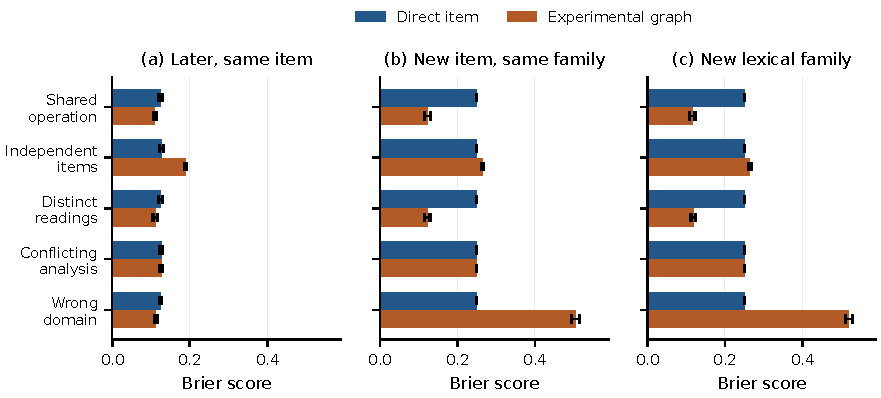
\includegraphics[width=\textwidth]{figures/prediction_brier.pdf}
\caption{Matched prediction comparison, lower Brier is better. Both estimators see identical observations and held-out outcomes. Error bars are sample SD across 12 fixed-seed means. The new-family split holds out independently assigned whole lexical families. Borrowing helps in the stipulated shared-operation world, does nothing under the conflict gate, and harms independent memorization and wrong-domain generalization. All data are synthetic.}
\label{fig:prediction}
\end{figure*}

Five worlds test this boundary. In \emph{shared operation}, a learner-specific probability is .1 or .9 across items. In \emph{independent memorization}, every item's probability is independently .1 or .9. \emph{Distinct readings} uses identical spelling with opposite probabilities for two reading IDs; joining by reading avoids spelling conflation. \emph{Conflicting analysis} disables borrowing. \emph{Wrong domain} reverses the probability for new-family and new-within-family items despite apparently supported metadata. Training-item performance can therefore look favorable while generalization fails.

For a binary held-out outcome $y_i$ and forecast $p_i$, we report Brier score $N^{-1}\sum_i(p_i-y_i)^2$, ten fixed equal-width-bin expected calibration error (ECE), and calibration curves. A forecast of at least .8 is called ``ready'' only for reporting. False-ready is failures among ready forecasts; coverage is ready forecasts divided by all questions. No ready forecasts means the conditional rate is undefined, not zero. Full counts, signed bias, and population false-ready rates are retained in JSON.

\begin{figure*}[t]
\centering
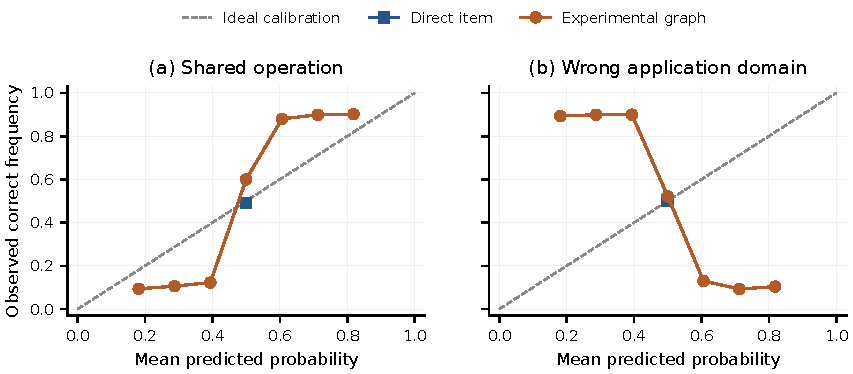
\includegraphics[width=.83\textwidth]{figures/calibration.pdf}
\caption{Pooled reliability bins for new lexical families. The diagonal denotes empirical agreement between forecast and outcome frequency. In the shared-operation world, direct predictions at .5 appear well calibrated in aggregate but distinguish no learners. The mixture improves Brier while remaining underconfident. Wrong-domain borrowing reverses the relationship and is severely miscalibrated. Markers show occupied bins, not uncertainty intervals.}
\label{fig:calibration}
\end{figure*}

\subsection{Matched-Budget Policy Comparison}

Both policies use the same direct estimator, six-item pool, and keyed common random numbers for response, help effect, and delayed outcome. Two items are task-critical with weight 4; the other four have weight 1. A question costs 20 seconds and help costs 40 seconds. Budgets are 60, 120, and 240 seconds. A fixed baseline already visits critical items first and always asks then helps, independent of correctness; it starts only complete 60-second episodes.

The diagnostic rule offers help below a .6 posterior-mean threshold and otherwise continues. It asks at most one question per item only when the correct and incorrect posterior branches change that action and the question plus potential help fit the remaining budget. Candidate scores use task-weighted expected decision value per second. A known gap can receive help directly. This is a fixed heuristic, not a learned policy or bandit, and its .6 action threshold differs from the .8 reporting threshold.

Help changes only simulated latent ability, never observed success counts:
\begin{align}
 p' &= p+gv(1-p),\qquad v\in[.8,1.2],\\
 p_{7d} &= p_0+r(p'-p_0).
\end{align}
The default assumed gain/retention pair is $(g,r)=(.45,.75)$; sensitivity uses $(.15,.50)$ and $(.65,.90)$. Baseline probability is otherwise fixed, except in the deliberately stale-history world. Assessments themselves cause no learning in this toy model, so the experiment does not test retrieval-practice theory. Every learner takes the same held-out tests seven days after the shared budget deadline. Unspent time remains ordinary chosen activity with no invented extra effect.

The five policy worlds are uncertain critical items, a known critical gap, already-ready items, misleading stale successes, and an assisted retry after a failure. Task success requires both critical held-out responses to be correct. We also report questions, help actions, interruptions, seconds used, calibration, and false-ready metrics. The identical estimator isolates the policy change; estimator misspecification remains shared.

\begin{figure*}[t]
\centering
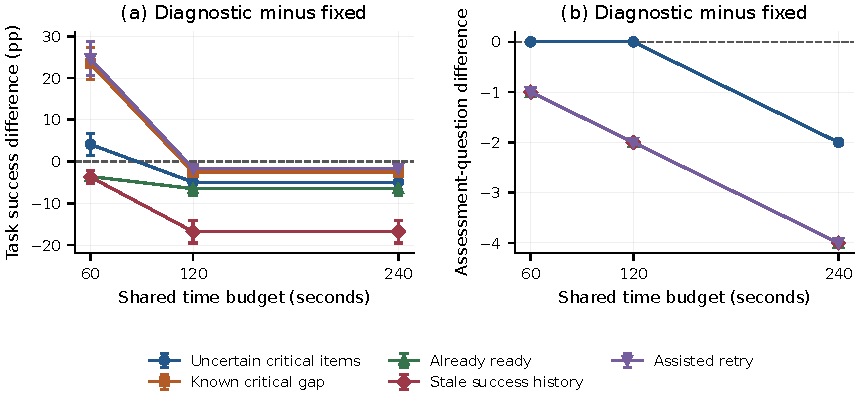
\includegraphics[width=\textwidth]{figures/policy_budget.pdf}
\caption{Diagnostic minus fixed-practice outcomes under the default assumed gain/retention regime. Left: paired task-success difference in percentage points; right: assessment-question difference. Both policies have the same estimator, item pool, costs, and shared time budget. Error bars are SD of paired differences across 12 seeds. Fewer questions can coexist with lower simulated success; unused task time is recorded without assigning it extra benefit.}
\label{fig:policy}
\end{figure*}

\section{Results and Counterexamples}
\label{sec:results}

\subsection{Structure Helps Only Under Suitable Assumptions}

Figure~\ref{fig:prediction} separates later-item, within-family, and new-family prediction. In the shared-operation new-family split, the direct model's Brier is $.2500\pm.0000$ and the experimental mixture's is $.1162\pm.0066$. Their paired difference is $-.1338\pm.0066$. This is an expected benefit when the generated world has exactly the common operation assumed by borrowing.

The independent-memorization world provides a counterexample even with structurally supported relationships. On later responses to trained items, direct Brier is $.1273\pm.0051$ and graph-informed Brier is $.1895\pm.0025$: pooling damages useful item-specific evidence. New-family error also increases, from .2500 to $.2637\pm.0039$. In the conflicting-analysis world, the two models agree exactly by construction. Distinct-reading new-family Brier is $.1186\pm.0061$ for the mixture; this result depends on the given reading IDs and does not establish an ability to infer readings from text.

The largest failure occurs under the wrong applicability domain. New-family Brier rises to $.5195\pm.0095$, a paired increase of $.2695\pm.0095$. Nevertheless, its later-trained-item score improves from .1244 to .1120. Evaluating only familiar items would obscure the failure. A well-formed structural relation and favorable in-domain accuracy do not establish learner-level transfer.

\subsection{Better Prediction Does Not Certify Calibration}

In shared-operation new-family prediction, direct ECE is .0263, versus .1393 for the mixture, despite the mixture's lower Brier (Figure~\ref{fig:calibration}). The direct constant .5 matches the approximately balanced marginal outcome. The mixture resolves some learner differences but shrinks predictions toward the middle. This is a calibration failure of the unfitted model, not a reason to prefer one summary metric universally.

At the .8 reporting threshold, the shared-operation mixture's new-family false-ready rate is $.0971\pm.0274$ with coverage $.2598\pm.0267$. Wrong-domain borrowing produces $.8963\pm.0234$ false-ready at $.2493\pm.0375$ coverage. Independent memorization gives $.3939\pm.1541$ conditional false-ready but only $.0130\pm.0084$ coverage; its small denominator makes that rate unstable. The direct new-family model never declares readiness, so its conditional false-ready rate is undefined. Reporting that rate as zero would conceal abstention.

\subsection{Diagnostic Value Depends on Budget and History}

At 60 seconds, diagnostic selection improves simulated task success for uncertain critical items by $4.10\pm2.58$ percentage points (pp), a known critical gap by $23.44\pm3.78$ pp, and an assisted-retry case by $24.61\pm4.06$ pp. The latter two need no extra uncertainty: direct evidence already favors useful help. In the known-gap world, the diagnostic rule spends 40 seconds on the weak second critical item; fixed practice first spends 60 seconds on the already-supported first item.

At 120 seconds, fixed practice can help both critical items, and the corresponding differences become $-4.95\pm1.71$, $-2.54\pm1.46$, and $-1.69\pm1.04$ pp. The values are unchanged at 240 seconds because additional fixed practice concerns noncritical items, while the diagnostic rule has already stopped. There is no universal diagnostic advantage (Figure~\ref{fig:policy}).

Stale successes are particularly harmful. With the shared stationary estimator, the diagnostic rule treats old strong evidence as sufficient and offers no corrective question or help. Its task-success deficit is $3.71\pm1.57$ pp at 60 seconds and $16.80\pm2.72$ pp at 120 seconds. The already-ready world also favors redundant fixed help under the assumed positive help effect, though that help introduces more interruptions. At 240 seconds, diagnostics ask two fewer questions in the uncertain-critical world and four fewer in each other world. Question reduction is a distinct outcome, not a proxy for learning.

Sensitivity to the declared gain/retention pairs is retained in Appendix~\ref{app:sensitivity}. No pair is estimated from learners. Both the reversals and the magnitude changes limit what these experiments can support: they test an action rule inside assumed worlds, not the effectiveness of \Nabu{}.

\section{Limitations, Impact, and an Unlaunched Pilot}
\label{sec:limits}

The synthetic worlds are intentionally small and favorable to interpretation, not representative of language learning. Binary outcomes omit attention, speech variation, contextual ambiguity, guessing strategies, correlated errors, and heterogeneous learning dynamics. Family independence, transfer applicability, 20/40-second costs, help effects, retention, and action utilities are assumptions. The graph mixture is not fitted or calibrated. Holding out entire declared families prevents one specific leakage, but does not make fictional families a linguistic benchmark. There are no human learning, usability, pronunciation, or retention results.

The production contract is conservative but incomplete. Assistance can be unobserved; correctly attributed events can still be noisy. Counts do not demonstrate independent evidence. An authored scorer can be wrong, and versions cannot repair a bad rubric automatically. The small contrast set does not identify lexical versus morphological causes conclusively. New analysis must be reviewable and stale evidence must be replayed explicitly. Unit and DOM checks verify specified behavior, not instruction quality or security under every deployment condition.

Privacy and autonomy matter because an intent may contain relationship, workplace, or other personal context. The new local parser sends no free-text intent to a third-party model. Evidence references intent revisions rather than repeating that text. Private member intent and organization objective remain distinct. Optional checks must not turn an exploratory reading into compulsory assessment or an employer-facing performance score. The current infrastructure does not justify claims of production-grade enterprise isolation.

A single proposed human pilot would use randomized parallel arms: fixed practice versus decision-sensitive optional diagnostics, each with a 12-minute session, the same independently reviewed Arabic material, estimator, candidate pool, and available assistance. Content and rubrics must be reviewed before recruitment; exact source, task, and scorer versions would be recorded. A blinded task-specific rubric would assess the primary task outcome, rather than clicks or completion alone. A delayed unaided check would target 48 hours, within a preregistered 42--54-hour window, using a genuinely changed sentence. Separate within-family and whole-new-family probes would be included only if independently reviewed eligible material exists; they would not be relabeled as each other. Baseline assessment would be separate from treatment observations. Declines, missing delayed responses, help uptake, interruption burden, and abandonment would be reported alongside performance, with a preregistered missingness analysis. The 12-minute budget and 48-hour target are design choices, not validated optima. Feasibility, measured costs, and outcome variability would inform a later trial's justified sample size. The full proposal accompanies the artifact as \artifact{docs/HUMAN_PILOT_PROPOSAL.md}. Approval and preregistration must precede recruitment. No study has been launched, and no sample-size, power, or efficacy claim is made here.

\section{Conclusion}

An intent can make help relevant without making competence identifiable. \Nabu{} now retains the conditions and provenance needed to examine that distinction, while preserving its existing reader and scheduler. The synthetic comparisons show why structural correctness, predictive accuracy, and intervention utility require separate tests: borrowing can mislead, calibration can fail, and a diagnostic policy can lose at a longer budget. The next empirical step is to validate assessments and costs, then test policy benefit under equal-time human conditions.

\label{mainbodyend}
\FloatBarrier
\raggedbottom
\bibliography{references}
\bibliographystyle{icml2026}

\clearpage
\appendix
\onecolumn
\section{Artifact, Reproduction, and Scope}
\label{app:artifact}

The paper accompanies a complete source delivery of the existing \Nabu{} repository with additive intent, structural safety, recommendation-input, and evidence features. The research scripts do not mutate production learner records, the language bank, the ontology, or the scheduler. The figures are vector PDFs regenerated directly from the saved result JSON. The figure manifest records the source SHA-256, protocol, seeds, and error-bar meaning. No data have been digitized from a chart or manually invented for presentation.

Run the following from the repository root using Node.js and Python with Matplotlib; compiling the paper additionally requires \texttt{pdflatex}, \texttt{bibtex}, and the included official style files.
\begin{verbatim}
node tools/evaluate_evidence.mjs --output docs/evidence-evaluation
node --test tests/evidence-evaluation.test.mjs
python tools/build_paper_figures.py
python tools/build_paper.py
\end{verbatim}

The recorded evaluation used Node.js 24.22.1. Its 22 focused research tests pass. A separate evidence-UI DOM suite uses the optional jsdom test dependency. These checks include duplicate handling, no passive evidence credit, split disjointness, prediction fairness, common policy constraints, all declared failure worlds, storage-error first-response freezing, lost-acknowledgement retry, actor/team changes, future records, and a complete optional contrast episode. These are scoped artifact checks, not a claim that unit tests establish linguistic or instructional validity. The main repository verification report records the final wider regression-suite totals separately.

The generator writes \texttt{docs/evidence-evaluation/results.json}, \texttt{results.csv}, and \texttt{report.md}. Two full runs of this protocol produced byte-identical versions of those files. The JSON contains configuration, family definitions, representation checks, nine research-semantic checks, nine production-projector checks, 360 per-seed prediction rows, 1,080 per-seed policy rows, aggregate metrics, paired deltas, selected traces, and explicit assumptions. There is no wall-clock timestamp in the generated results. Changed source or runtime can change hashes; the result metadata records both.

\subsection{Implementation Boundaries}

\begin{tabular}{@{}>{\raggedright\arraybackslash}p{.34\textwidth}>{\raggedright\arraybackslash}p{.61\textwidth}@{}}
\toprule
Artifact & Responsibility and boundary \\
\midrule
\artifact{public/nabu-intents.js} and store/UI & Conservative intent parsing and editable provenance; separate private learner intent and organization objective. \\
\artifact{public/nabu-structure.js} & Typed compatibility bridge over existing alignment data; provenance and quality gates, no invented multilingual lexemes or imported morphology. \\
\artifact{public/nabu-observations.js} & Strict envelope/sequence validation and pure actor-scoped evidence projection; no I/O, graph transfer, scheduler, or competence probability. \\
\artifact{public/nabu-evidence-tasks.js} & Exact authored task/scoring versions and contrast prerequisites; draft status is retained. \\
\artifact{public/nabu-evidence-policy.js} & Deterministic help/check/continue choices with transparent outcome branches; no bandit or measured gain. \\
\artifact{public/nabu-evidence-ui.js} & Optional reader controls, immutable response saves, replay and export; preserves existing source and learning state. \\
\artifact{tools/evaluate_evidence.mjs} & Separate assumed Beta/mixture models and synthetic worlds; never installs a production learner posterior. \\
\bottomrule
\end{tabular}

\section{Exact Synthetic Prediction Protocol}
\label{app:prediction}

\subsection{Fixed Seeds and Family Manifest}

The 12 seeds are $11,29,47,83,101,137,173,211,257,307,359,419$. Each world has 128 generated learners per seed. These values are specified in source, not chosen after comparing outcomes. Pseudorandom values are deterministic hashes of seed, world, learner, item, and event-role keys; the same key produces the same potential outcome for both compared policies. The function is a reproducibility device, not a cryptographic random generator or an assertion of statistical independence in real data.

\begin{table}[ht]
\caption{Independently assigned fictional lexical-family IDs. Every family has members \texttt{a}, \texttt{b}, and \texttt{c}; the partition applies to all of them. The labels are mnemonic fixture labels, not natural-language lemmas.}
\centering
\begin{tabular}{llll}
\toprule
Observed family & Fixture label & Fully held-out family & Fixture label \\
\midrule
\texttt{lexfam-113} & amber & \texttt{lexfam-719} & glen \\
\texttt{lexfam-227} & birch & \texttt{lexfam-823} & heath \\
\texttt{lexfam-349} & cobalt & \texttt{lexfam-941} & iris \\
\texttt{lexfam-461} & dune & \texttt{lexfam-1061} & jade \\
\texttt{lexfam-587} & elm & \texttt{lexfam-1171} & kelp \\
\texttt{lexfam-601} & flint & \texttt{lexfam-1283} & larch \\
\bottomrule
\end{tabular}
\end{table}

Training includes $6\times2\times3=36$ binary responses per learner. The three held-out splits have 12, 6, and 6 questions, respectively. Across 1,536 fictional learners per world, they contain 18,432, 9,216, and 9,216 questions. There are 184,320 distinct held-out outcomes across five worlds, scored by both models. This is 368,640 forecasts, not 368,640 independent observations.

The experimental model sorts eligible source events by identifier and takes the first one from each other family. Selecting one event per declared family limits reuse; it does not establish real-world independent sources. The family independence claimed in the research result is stipulated by the simulation. A spelling identity never supplies a join. In the distinct-reading world, slot \texttt{a} uses reading A and the other slots use reading B, with opposite latent response probabilities. The target family is always excluded from borrowed evidence, including when the target is a held-out \texttt{c} of an observed family.

\subsection{Metrics and Denominators}

For ten bins $B_b=[b/10,(b+1)/10)$, with probability 1 included in the final bin,
\begin{equation}
 \operatorname{ECE}=\sum_{b:|B_b|>0}\frac{|B_b|}{N}
 \left|\frac{\sum_{i\in B_b}p_i}{|B_b|}-\frac{\sum_{i\in B_b}y_i}{|B_b|}\right|.
\end{equation}
Signed calibration bias is $N^{-1}\sum_i(p_i-y_i)$. At threshold $\tau=.8$, ready coverage is $N^{-1}\sum_i\ind[p_i\ge\tau]$; conditional false-ready is $\sum_i\ind[p_i\ge\tau,y_i=0]/\sum_i\ind[p_i\ge\tau]$ when the denominator is positive. Population false-ready divides the same numerator by $N$. Conditional summaries omit undefined seeds and report their defined-seed count in JSON. Pooled calibration curves use all questions in a world/split; reported mean ECE instead averages per-seed ECE. These aggregations are not interchangeable.

\begin{table}[ht]
\caption{New-family prediction results. Values are means $\pm$ sample SD across 12 seeds. The direct model always predicts .5 on this split, giving Brier .2500 and zero ready coverage. All entries are synthetic.}
\centering
\begin{tabular}{lrrrr}
\toprule
World & Mixture Brier & Paired Brier change & Mixture false-ready & Mixture ready coverage \\
\midrule
Shared operation & $.1162\pm.0066$ & $-.1338\pm.0066$ & $.0971\pm.0274$ & $.2598\pm.0267$ \\
Independent memorization & $.2637\pm.0039$ & $+.0137\pm.0039$ & $.3939\pm.1541$ & $.0130\pm.0084$ \\
Distinct readings & $.1186\pm.0061$ & $-.1314\pm.0061$ & $.0966\pm.0228$ & $.2441\pm.0332$ \\
Conflicting analysis & $.2500\pm.0000$ & $.0000\pm.0000$ & undefined & $.0000\pm.0000$ \\
Wrong domain & $.5195\pm.0095$ & $+.2695\pm.0095$ & $.8963\pm.0234$ & $.2493\pm.0375$ \\
\bottomrule
\end{tabular}
\end{table}

\section{Policy Rule and Sensitivity}
\label{app:sensitivity}

For an item with Beta parameters $(\alpha,\beta)$, the two hypothetical posterior means are $(\alpha+1)/(\alpha+\beta+1)$ and $\alpha/(\alpha+\beta+1)$. Let $d(p)=\max(0,.6-p)$ and let $w_j\in\{1,4\}$ be the task weight. A question candidate exists only when the two posterior means yield different help/continue actions, it has not already been asked, and at least 60 seconds remain. Its score is
\begin{equation}
 \frac{w_j}{20}\left[p\,d(p_{\mathrm{correct}})+(1-p)\,d(p_{\mathrm{incorrect}})-d(p)\right].
\end{equation}
A help candidate exists when $p<.6$, the item has not already been helped, and 40 seconds remain; its score is $w_j(.6-p)/40$. Where an eligible question is considered for an item, direct help for that item is deferred until the outcome. Ties are broken deterministically by item ID. At most one question and one help action occur per item. This threshold-value heuristic is intentionally simple and is not an optimal policy for the simulator's help dynamics.

The first two pool items are critical. Default supported items have 12 historical successes, one failure, and current probability .85. In the uncertain-critical world, both critical items have no history and probability .15 or .85. A known critical gap has one success, 15 failures, and probability .15 on the second critical item. Already-ready items have 12 successes, no failures, and probability .9. Stale-history critical items have the same strong history but current probability .15; noncritical probability is .9. In the assisted-retry world, the second critical item has one unaided failure, a help event, and an assisted correct retry, with probability .15. The retry cannot turn its history into a success.

\begin{figure}[ht]
\centering
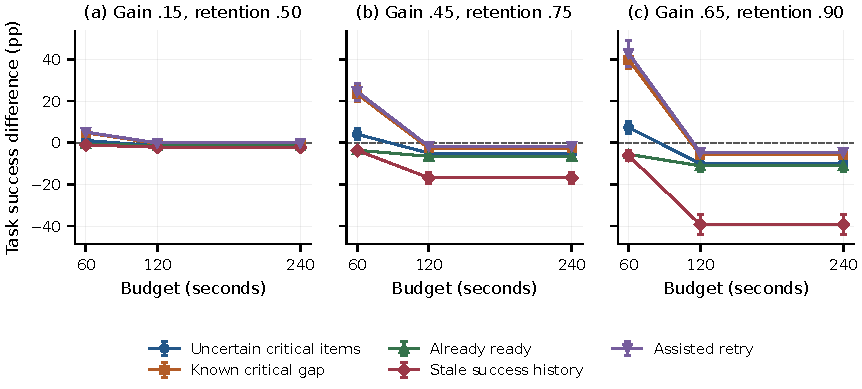
\includegraphics[width=\textwidth]{figures/policy_sensitivity.pdf}
\caption{Sensitivity to assumed learning and retained gain. Each panel repeats the same policy comparison and common random numbers under a different declared $(g,r)$ pair. Values are diagnostic minus fixed task success; error bars are sample SD across seeds. The experiments show assumption-dependent magnitudes and budget reversals, not fitted human retention.}
\end{figure}

The simulator records the number of questions and help actions separately; ``interruptions'' is their sum. A question followed by help is therefore two action-level interruptions, not necessarily two separate reader sessions. Both policies have the same maximum wall-clock support budget; neither is forced to consume it. The unused seconds are recorded, not credited with additional hypothetical learning. Fixed practice may continue to noncritical items at 240 seconds, which affects its question count and all-item calibration but not the critical-item task-success definition. Both policies face the same six terminal test items after the common deadline.

\section{Authored Contrast Sequence and Assessment Boundaries}
\label{app:contrasts}

\begin{table}[ht]
\caption{The small production contrast set. The labels describe task purposes, not validated diagnoses. Supplied cues remain assistance; the source is preserved while a check is open. No new audio recording is fabricated.}
\centering
\begin{tabular}{p{.17\textwidth}p{.35\textwidth}p{.39\textwidth}}
\toprule
Task key & What is presented & Boundary of an assessment \\
\midrule
\texttt{take-meaning} & Choice of base meaning: take, give, or write & Visual meaning recognition; no free-production or listening claim \\
\texttt{open-meaning} & Recognition of the other base meaning & Establishes direct evidence for that base before its operation check \\
\texttt{take-female} & Addressed form with base meaning supplied & Supplied meaning makes the response assisted \\
\texttt{open-female} & Operation on the other, directly checked base & A response under this recorded base and cue condition \\
\texttt{take-male} & Opposite address-direction contrast & A distinct target; success does not overwrite the first direction \\
\texttt{write-female} & A further base with meaning supplied & Assisted application on this base, not generalized operation mastery \\
\texttt{phrase-now} & Phrase completion in the current context & Contextual task response; does not establish delayed retention \\
\texttt{phrase-later} & Different sentence after a prior direct check and at least 24 hours & Exact delay and changed tested condition, not a fitted retention rate \\
\bottomrule
\end{tabular}
\end{table}

Legacy activity behavior is preserved. A previously identified mismatch between an old poem prompt and its annotation is not silently corrected by treating its recorded result as reliable evidence: the new resolver leaves that legacy interpretation unscored. The ledger retains the reason. This illustrates the role of versioned source and scoring references: provenance enables review, but does not certify that authored content is correct.

\FloatBarrier
\section{Proof Boundaries and Failure Cases}
\label{app:proofs}

Proposition~\ref{prop:replay} is scoped to validated enveloped events for the selected actor and team. Events for other actors are ignored before their conflicts affect the selected projection. Exact equality is canonical object equality, independent of object property order. It does not collapse distinct event IDs with similar content: doing so would lose real repeats. Episode validation rejects contradictory retry parents and attempt identities; unresolved retry ancestry cannot receive fresh credit. The pure resolver/scorer condition matters because a time-varying or stochastic scorer would invalidate deterministic replay.

There are two explicit non-monotonicities. A newly recorded hint or visible answer can reveal that an earlier apparent success was assisted; adding it may reduce direct credit. A changed rubric or analysis can make an event stale until an explicit rescore. Neither is a historical event mutation. An audit consumer must retain original observations and treat a projection as version- and policy-dependent. A tied timestamp between distinct earliest responses does not license arbitrary ordering; both abstain. Same-attempt feedback recorded at the response instant is not used retroactively as help for that first response.

Proposition~\ref{prop:nonidentifiable} is a counterexample to identification from passive data alone, not a prohibition against all inference from skips, help seeking, or exposure. Such inference would require an explicit, empirically defensible observation model and a declared target population. In the two-world construction, the observation mechanism is identical and independent of the differing latent response probabilities. Any procedure forced to output a single probability must therefore be wrong in at least one world. Returning unknown is an admissible production choice; the separate research estimator's .5 prior is an assumption, not an observed fact.

\end{document}
